\documentclass[border=3pt]{standalone}
\usepackage{tikz}
\usetikzlibrary{arrows.meta,calc}
\tikzset{pin/.style={-{Stealth[length=5pt]}}}
\begin{document}
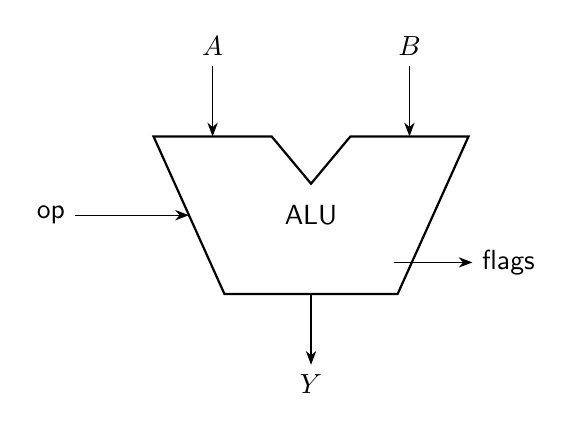
\begin{tikzpicture}[font=\sffamily]
  % classic ALU shape: wide notched top, narrow bottom
  \draw[thick]
    (0,2) -- (1.5,2) -- (2.0,1.4) -- (2.5,2) -- (4,2)
    -- (3.1,0) -- (0.9,0) -- cycle;
  \node[font=\sffamily] at (2,1.0) {ALU};
  % operand inputs (top)
  \draw[pin] ($(0.75,2.0)+(0,9mm)$) node[above]{$A$} -- (0.75,2.0);
  \draw[pin] ($(3.25,2.0)+(0,9mm)$) node[above]{$B$} -- (3.25,2.0);
  % op select (left)
  \draw[pin] (-1.0,1.0) node[left]{op} -- (0.45,1.0);
  % result (bottom)
  \draw[pin] (2,0) -- ++(0,-9mm) node[below]{$Y$};
  % flags (right)
  \draw[pin] (3.05,0.4) -- ++(10mm,0) node[right]{flags};
\end{tikzpicture}
\end{document}
